% CVPR 2026 main-track draft — ConFu++
% Official cvpr.sty (cvpr-org/author-kit). Every number traces to this
% repository's experimental record (EXPERIMENTS.md + results/ JSONs).
\documentclass[10pt,twocolumn,letterpaper]{article}
\usepackage[review]{cvpr}
\usepackage{times}
\usepackage{epsfig}
\usepackage{graphicx}
\usepackage{amsmath,amssymb}
\usepackage{booktabs,multirow,array}

\usepackage{xcolor}
\usepackage[hidelinks]{hyperref}

\newcommand{\rI}{r_{12}}
\newcommand{\ro}{r_1}
\newcommand{\rt}{r_2}
\newcommand{\pp}{\,pp}
\def\cvprPaperID{0000}
\def\paperID{0000}
\def\confName{CVPR}
\def\confYear{2026}

\title{Alignment Is Not Dependence:\\Measuring and Reducing Unimodal Shortcuts in\\Higher-Order Multimodal Fusion}

\author{Anonymous CVPR submission\\
\paperID{\cvprPaperID}}

\begin{document}
\maketitle

\begin{abstract}
Higher-order multimodal methods fuse per-modality encodings and align them contrastively, on the
premise that fused representations capture information unavailable to any constituent modality.
We show this premise is empirically unfounded. Across AV-MNIST, CMU-MOSI, and UR-FUNNY,
interaction representations that are active, predictive, high-rank, and permutation-sensitive are
nevertheless almost entirely predictable from a single modality (nonlinear predictability up to
$R^2=0.989$). We formalize this \emph{alignment--dependence gap} and introduce an operational
diagnostic suite separating fusion, dependence, and conditional utility. We then propose
\textbf{ConFu++}: a conditional-utility objective plus \textbf{S1}, an adversarial
de-shortcutting penalty acting on the interaction at training time --- taxing predictability from
each single modality while leaving joint predictability unconstrained. S1 is the only objective
among those studied that significantly reduces the measured shortcut (paired $p\approx0.011$,
five seeds) at zero accuracy cost, and it fabricates no dependence on negative controls. On a
controlled synthetic benchmark with ground-truth third-order synergy, order-restricted models sit
at chance while an order-matched interaction solves the task with perfectly balanced dependence
($+49.9$\pp, 5/5 seeds). On the newly released Bird-MML benchmark --- which our audit shows to
contain genuine image--text headroom --- the original objective captures none of it
($+0.2$\pp\ of $+15.9$\pp available), while ConFu++ recovers a significant share
($+5.76{\pm}0.86$\pp, paired $p<0.001$). We further document two transferable pitfalls:
post-aggregation LayerNorm leaks higher-order signal (invalidating ``low-order'' ablations), and
online adversaries equilibrate far below converged probes. Code, diagnostics, the synthetic
benchmark, and all experiment logs will be released.
\end{abstract}

\section{Introduction}
Multimodal representation learning increasingly builds joint representations by fusing
per-modality encodings and aligning them with contrastive objectives
\cite{clip,symile,imagebind,confu}. The tacit assumption: fusion \emph{integrates} the
modalities. We ask a question the literature rarely answers directly --- does the fused
representation actually \emph{depend} on all of its inputs?

Figure~\ref{fig:teaser} summarizes our central finding on AV-MNIST: an interaction representation
that is non-collapsed, high-rank, predictive, and permutation-sensitive is simultaneously a near
pure function of the image modality ($R^2(\ro\!\to\!\rI)=0.989$; audio: $0.031$). Nothing in the
training objective forbids this. We argue this \emph{alignment--dependence gap} is systematic,
measurable, and --- on current benchmarks --- nearly universal.

Our study proceeds in four steps. \textbf{(i) Formalism and diagnostics}
(\S\ref{sec:gap}): we define activity, dependence, and conditional utility operationally, and
assemble a diagnostic battery (zero-vs-shuffle, per-modality corruption, capacity-matched
conditional probes, correction--regression, predictability probes). \textbf{(ii) Audits}
(\S\ref{sec:audit}): three standard benchmarks fail either the dependence or the utility gate;
we log all failed repair attempts as negative results. \textbf{(iii) Method}
(\S\ref{sec:method}): ConFu++ couples a conditional-utility margin with S1, a hinged adversarial
penalty on single-modality predictability of the interaction. \textbf{(iv) Controlled ground
truth} (\S\ref{sec:synthetic}): on synthetic tasks with known latent structure, we verify the
mechanism is sound (learns synergy when present), honest (fabricates none when absent), and that
order-matched interactions are necessary and sufficient for third-order synergy.
\textbf{(v) Natural positive} (\S\ref{sec:birdmml}): on Bird-MML, which our audit shows contains
genuine image--text complementarity, ConFu++ improves the original objective by
$+5.76{\pm}0.86$\pp\ ($p<0.001$, five seeds), exceeding the raw-feature probe ceiling.

\begin{figure}[t]
\centering
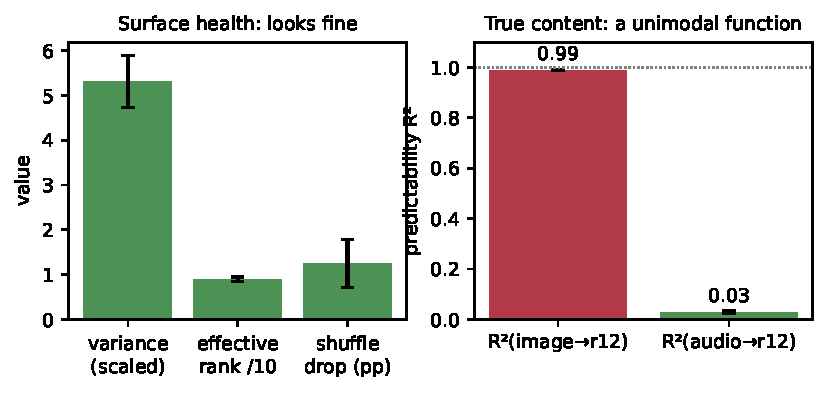
\includegraphics[width=\columnwidth]{figures/fig1_avmnist_paradox.pdf}
\caption{\textbf{The AV-MNIST paradox.} Left: by every surface criterion (variance, effective
rank, shuffle sensitivity) the interaction $\rI$ looks healthy. Right: a nonlinear probe recovers
$\rI$ almost perfectly from the image alone. Joint computation $\neq$ joint information.
Five seeds; bars show mean$\pm$std.}
\label{fig:teaser}
\end{figure}

\section{Related Work}
\paragraph{Contrastive multimodal alignment.}
CLIP \cite{clip} popularized pairwise InfoNCE alignment; Symile \cite{symile} extends it to three
or more modalities via a total-correlation bound; TriCLIP and ImageBind \cite{imagebind} bind
multiple modalities through shared anchors. ConFu \cite{confu}, our direct baseline, aligns fused
pair representations with the remaining modality. None of these objectives constrains the
\emph{content} of the fused representation --- our predictability probes apply to all of them.

\paragraph{Fusion architectures.}
Multiplicative and tensor fusion (MFN, LMF \cite{lmf}), cross-modal transformers (MUL-T), and
disentangled variants (MISA) optimize the \emph{capacity to fuse}. We instead measure whether the
fusion \emph{depends} on its inputs --- an orthogonal axis, and the one that fails first.

\paragraph{Modality dominance and shortcuts.}
Multimodal networks overfit and one modality often dominates \cite{wang2020}; gradient
rebalancing (OGM-GE \cite{ogm}) and modality dropout react at the loss/gradient level;
underspecification \cite{underspec} frames the general phenomenon. Our root-cause analysis shows
why loss-level pressure cannot bootstrap dependence: under a shortcut, corrupted and positive
interactions coincide, so the ranking/margin signal vanishes exactly where it is needed. We
compare against an OGM-style baseline on identical frozen features (\S\ref{sec:birdmml}).

\paragraph{Synergy and information decomposition.}
Partial information decomposition \cite{pid} supplies the vocabulary (unique, redundant,
synergistic information); MultiViz \cite{multiviz} operationalizes interaction importance via
perturbation. \emph{Relation to PID:} our predictability-based quantities are operational bounds,
not PID estimates --- a representation can be unpredictable from $\ro$ alone yet carry no
unique information about $Y$, and vice versa. We use PID only as motivation; every claim rests on
the operational definitions of \S\ref{sec:gap}, whose limitations we state explicitly.

\paragraph{Adversarial representation control.}
Domain-adversarial training \cite{dann} and ``learning not to learn'' \cite{learningnottoplearn}
remove unwanted predictability. S1 differs in target: predictability of the \emph{interaction}
from \emph{each constituent alone} --- never from the pair jointly --- with a hinge that avoids
the degenerate noise solution. Anti-collapse terms follow VICReg \cite{vicreg}.

\section{The Alignment--Dependence Gap}\label{sec:gap}
\textbf{Setup.} Encoders $E_i$ produce $r_i=E_i(X_i)$; a fusion module produces
$\rI=F(\ro,\rt)$. We separate four properties:
\begin{itemize}\itemsep2pt
\item \textbf{Active}: $\mathrm{Var}(\rI)>0$ (diagnosed by variance floor and effective rank);
\item \textbf{Predictive}: $I(Y;\rI)>0$, approximated by standalone probes;
\item \textbf{Dependent}: corrupting either constituent before fusion degrades performance
($D_1>0$ and $D_2>0$);
\item \textbf{Conditionally useful}:
$\mathrm{Perf}(\ro,\rt,\rI)>\mathrm{Perf}(\ro,\rt)$.
\end{itemize}
An interaction is \emph{complementary} only when both of the last two hold. The central
observation: contrastive alignment ($\rI\!\leftrightarrow\!r_3$) and task cross-entropy are
\emph{both} satisfied by the shortcut $\rI\approx f(\ro)$, through three escape routes ---
strong-factor dominance in multiplicative fusion, nonlinear copying invisible to covariance
penalties, and classifier-side bypass through gated composition.

\textbf{Diagnostic suite.}
(i) \emph{Zero vs.\ shuffle}: zeroing $\rI$ measures necessity; shuffling it measures mismatch
sensitivity --- a positive shuffle drop alone is not utility evidence (mismatched interactions
act as adversarial perturbations). (ii) \emph{Per-modality corruption}: shuffle modality $i$
\emph{before} computing $\rI$; drops $D_i$ and balance
$B_{12}=2\min(D_1,D_2)/(D_1+D_2)$. (iii) \emph{Conditional probes}: capacity-matched linear and
nonlinear probes on $[\ro,\rt]$ vs.\ $[\ro,\rt,\rI]$. (iv) \emph{Correction--regression}:
per-sample win/loss counts of full vs.\ lower-order predictions. (v) \emph{Predictability
probes}: converged nonlinear $q_1(\ro)\!\to\!\rI$, $q_2(\rt)\!\to\!\rI$,
$q_{12}(\ro,\rt)\!\to\!\rI$ with the shortcut criterion $R^2(q_1)\gg R^2(q_2)$ and
$R^2(q_1)\approx R^2(q_{12})$.

\section{ConFu++}\label{sec:method}
\begin{figure}[t]
\centering
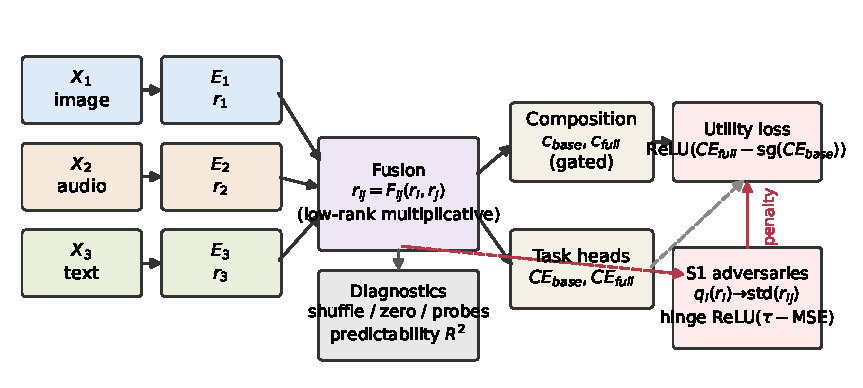
\includegraphics[width=\columnwidth]{figures/fig2_pipeline.pdf}
\caption{\textbf{ConFu++}. Contrastive fusion plus two training-time objectives:
conditional utility (top right) and S1 adversarial de-shortcutting (bottom right). Adversaries
and probes are training-only; inference capacity is unchanged.}
\label{fig:pipeline}
\end{figure}

\textbf{Composition.} Following the validated baseline, $c_{base}=\mathrm{LN}(\mathrm{LN}(\ro)+
\mathrm{LN}(\rt))$ and $c_{full}=\mathrm{LN}(c_{base}+\sigma(a)\,\mathrm{LN}(\rI))$, with
$\rI=W_o\,\frac{u_1\odot u_2}{\sqrt{R}}$, $u_i=\mathrm{LN}(U_i r_i)$ (low-rank multiplicative
interaction, rank $R$).

\textbf{Conditional utility.} Per-sample margin against the detached lower-order loss:
$L_{util}=\mathrm{ReLU}(CE_{full}-\mathrm{sg}(CE_{base})+m)$, weight $0.2$, $m{=}0$.

\textbf{S1: adversarial de-shortcutting.} Let $t=\mathrm{std}(\rI)$ with stop-grad EMA
statistics. Adversaries $q_1,q_2$ (MLPs capacity-matched to the evaluation probe) minimize
$\|q_i(r_i)-t\|^2$ in an alternating step; the generator pays the hinged penalty
\begin{equation}
L_{shortcut}=\sum_{i=1,2}\mathrm{ReLU}\!\big(\tau-\mathrm{MSE}(q_i(r_i),t)\big),
\end{equation}
with gradient flowing through $t$ only. Because $t$ is standardized, MSE equals $1{-}R^2$ of the
adversary: the hinge taxes single-modality $R^2$ above $1{-}\tau$ and then switches off, so the
task loss never trades against noise-making. Crucially, \emph{no} adversary sees the pair ---
joint predictability is intended. Per-factor variance floors close the constant-factor escape
route. Warmup over the first 10--20\% of epochs; $k_{adv}{=}1$; adversary LR $0.5\times$.


\begin{figure}[t]
\fbox{\parbox{0.97\columnwidth}{\small
\textbf{Algorithm 1: ConFu++ training step (per batch).}\\[2pt]
\textbf{Input:} batch $(X_1,X_2,y)$; encoders $E_i$; interaction $F$; heads; adversaries
$q_1,q_2$; EMA stats $(\mu,\sigma)$.\\[2pt]
1.\quad Encode: $r_i{=}E_i(X_i)$; $r_{12}{=}F(r_1,r_2)$; $c_{base}$, $c_{full}$.\\
2.\quad \emph{Adversary step:} $t{=}\mathrm{sg}[\mathrm{std}(\rI)]$; update $q_1,q_2$ on
$\|q_i(r_i){-}t\|^2$ (all encoders frozen).\\
3.\quad \emph{Generator step:} with frozen $q_i$, update the generator on
$L{=}CE_{full}{+}\lambda_u L_{util}{+}\lambda_{var}L_{var}{+}\lambda_{cov}L_{cov}{+}L_{S1}$,
where $L_{S1}{=}\lambda_{s1}\,\mathrm{warmup}\,\sum_i \mathrm{ReLU}(\tau{-}\mathrm{MSE}(q_i(r_i),t))$;\\
\quad\quad plus per-factor variance floors; gradient clip $1.0$; generator params only.\\
4.\quad Update EMA $(\mu,\sigma)$; log adversary MSEs (the live shortcut meter).
}}
\caption{Alternating minimax of ConFu++. Steps 2 and 3 never share gradients.\vspace{-6pt}}
\label{fig:alg}
\end{figure}

\textbf{Honesty by construction.} Where a modality carries nothing, the correct outcome is no
dependence --- S1 must report exactly that. We treat fabricated dependence on negative controls
as a failure of the method, not a win.

\section{Auditing Existing Benchmarks}\label{sec:audit}
\begin{table}[t]\centering\small
\caption{Five-seed audits of higher-order interactions. Surface metrics pass everywhere;
dependence/utility gates fail everywhere.}
\label{tab:audit}
\resizebox{\columnwidth}{!}{\begin{tabular}{@{}lccc@{}}
\toprule
 & AV-MNIST & CMU-MOSI & UR-FUNNY \\
\midrule
Dominant modality & image & text & text \\
$R^2$ (best single $\to$ interaction) & 0.989 & 0.953 & 0.970 \\
Weak-modality shuffle drop (pp) & $+0.004$ & --- & --- \\
Pair conditional gains (pp) & $+0.02$ & $-0.96/-1.43/-2.27$ & $-0.66/+0.19/-0.76$ \\
\bottomrule
\end{tabular}}
\end{table}

Table~\ref{tab:audit} condenses three five-seed audits (full per-seed logs in the supplement).
On AV-MNIST, shuffling audio before the interaction costs $+0.004{\pm}0.027$\pp\ --- the
interaction is effectively image-only. On MOSI, text dominates and all pair conditional gains are
negative. On UR-FUNNY, pair interactions are active and permutation-sensitive yet linearly
redundant ($R^2\approx0.97$ from lower-order inputs). We additionally logged two failed repairs:
a conditional-utility objective alone (P1) raised nonlinear conditional gain but not dependence,
and a task-aware ranking objective (P2) collapsed --- under a shortcut, corrupted and positive
interactions coincide, so the ranking signal vanishes where it is needed. This failure mode is
itself evidence for the gap.

\textbf{Not ConFu-specific.} A CLIP-lineage control (pairwise InfoNCE only, identical fusion
heads, Bird-MML frozen features, 5 seeds) shows the same shortcut: $R^2(\mathrm{image}\to
z_{12})=0.99$, $R^2(\mathrm{text}\to z_{23})=0.99$ --- fused heads converge to single-modality
functions even without any higher-order alignment term. The gap is a property of the
contrastive-alignment lineage, not of one objective.

\textbf{Verdict.} Current natural benchmarks in this family exhibit \emph{information absence or
dominance}. No training objective can create missing information; the correct scientific response
is (a) measure it, (b) verify the mechanism where ground truth exists, (c) find a benchmark with
validated headroom.

\section{Controlled Order Benchmark}\label{sec:synthetic}
\begin{figure}[t]
\centering
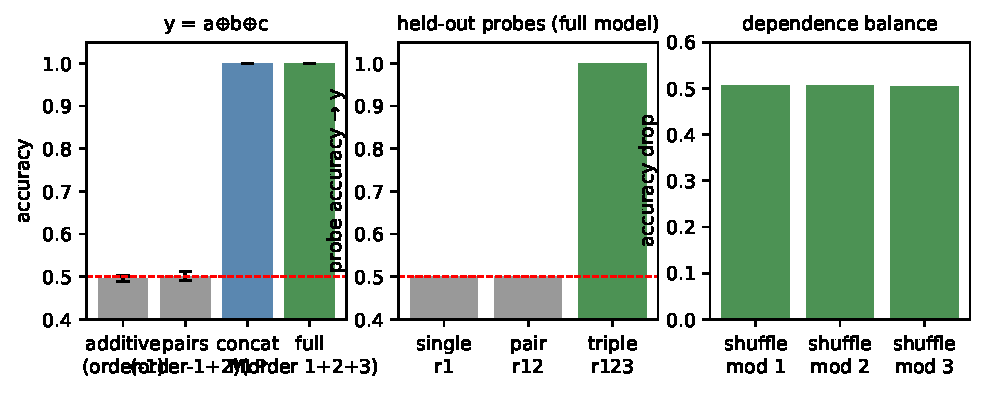
\includegraphics[width=\columnwidth]{figures/fig4_order3.pdf}
\caption{\textbf{Order-3 synergy} ($y{=}a{\oplus}b{\oplus}c$). Left: only the order-matched model
exceeds chance (5 seeds). Middle: held-out probes of the full model --- singles and pairs at
chance, $r_{123}$ perfect. Right: corrupting any single modality costs ${\approx}0.5$ accuracy.}
\label{fig:order3}
\end{figure}

We construct tasks with known latent structure: each modality observes an independent latent bit
through a fixed random prototype plus Gaussian noise (50k train / 4k test; 5 seeds). Labels:
order-2 $y{=}a{\oplus}b$ with a distractor modality (honesty control), order-3
$y{=}a{\oplus}b{\oplus}c$ (pure third-order synergy --- independent of every single modality and
every pair), and a routed mixture (an observable flag selects between a unimodal rule and the XOR
rule; Bayes = 1.0).

\begin{table}[t]\centering\small
\caption{Order-3 benchmark: accuracy (5 seeds). Order-restricted decompositions are at chance;
the order-matched interaction solves the task with balanced dependence.}
\label{tab:order3}
\resizebox{\columnwidth}{!}{\begin{tabular}{@{}lccc@{}}
\toprule
Model & orders & accuracy & min shuffle drop \\
\midrule
Additive & 1 & $0.496{\pm}0.006$ & $-0.007$ \\
Pairs-only & 1+2 & $0.501{\pm}0.010$ & $-0.007$ \\
Concat-MLP (joint) & all & $1.000{\pm}0.000$ & $+0.501$ \\
\textbf{Full (order 1+2+3)} & 1+2+3 & $\mathbf{1.000{\pm}0.000}$ & $+0.501$ \\
\bottomrule
\end{tabular}}
\end{table}

Three findings stand out. \textbf{(1) Necessity and sufficiency}: order-restricted models sit at
chance while the order-matched term is perfect (Table~\ref{tab:order3},
Fig.~\ref{fig:order3}). \textbf{(2) Readout, not information}: pair representations do contain
the bits (concat-pair probe $0.97$), yet the sum-aggregated order-2 model stays at chance ---
higher-order synergy requires order-matched \emph{computation}, not merely rich features.
\textbf{(3) Scaling}: the $M$-ladder ($M{=}3..6$, Fig.~\ref{fig:ladder}a) keeps
order-restricted models at chance at every $M$ while the full model solves all of them with
min-drop ${\approx}{+}0.5$; concat-MLP begins to crack at $M{=}6$ ($0.9975$).

\textbf{S1 on ground truth.} With synergy present (Config A), S1 preserves accuracy (1.000) and
halves single-modality predictability of $\rI$; with synergy absent (Config B) it fabricates
nothing (all drops ${\approx}0$). On the routed mixture, all variants solve the task; under an
epoch budget the hard-fraction emphasis variant (S4) raises the XOR-fraction accuracy
($0.92{\to}0.97$) but trades easy-fraction accuracy --- documented as exploratory-negative.

\section{Bird-MML: A Natural Benchmark with Genuine Headroom}\label{sec:birdmml}
Bird-MML \cite{confu} (Zenodo 18920487) pairs bird photos, audio clips, and captions for 149
species. The release's audio archive is missing one part (all present parts MD5-verify); we
recover a balanced 71-species, 70{,}796-row tri-modal subset with a fixed stratified split ---
identical for every compared method.

\paragraph{Audit.} Frozen features (ResNet50 / wav2vec2 / MiniLM) reveal exactly one strong pair:
image+text reaches $80.89\%$ vs.\ best single $64.95\%$ ($+15.94$\pp\ headroom), while audio
carries nothing (1.43\%, chance). Leakage audit: 33\% of captions contain the species name; a
BLIP-only (name-free) control reduces headroom to $+4.78$\pp\ --- still positive, so genuine
complementarity survives de-leakage. The audio-null result is robust across speech- and
AudioSet-domain extractors (AST re-audit: $+0.35$\pp).

\begin{table}[t]\centering\small
\caption{Bird-MML frozen-feature matrix (5 seeds, paired).}
\label{tab:bird}
\resizebox{\columnwidth}{!}{\begin{tabular}{@{}lcccc@{}}
\toprule
 & ConFu & +S1 & +U & +U+S1 \\
\midrule
probe full (\%) & $76.90{\pm}.65$ & $76.58{\pm}.51$ & $83.01{\pm}.13$ & $82.66{\pm}.37$ \\
cond.\ gain (pp) & $+0.19$ & $-0.36$ & $+1.07$ & $+0.77$ \\
$R^2(\mathrm{text}{\to}z_{13})$ & $0.59$ & $0.69$ & $\mathbf{0.44}$ & $0.50$ \\
audio drop (pp) & $+0.01$ & $+0.01$ & $+0.01$ & $+0.01$ \\
\bottomrule
\end{tabular}}
\end{table}

\paragraph{Result.} The original objective captures none of the available complementarity
(full ${\approx}$ lower; $+0.19$\pp). ConFu+U recovers $83.01\%$ and ConFu+U+S1
$82.66{\pm}0.37\%$: paired against the original, $+5.76{\pm}0.86$\pp\ ($t{=}14.91$,
$p{<}0.001$), above the raw-feature linear ceiling ($81.01\%$). Attribution is explicit
(Table~\ref{tab:bird}): the accuracy gain comes from the utility objective; S1's contribution is
representation quality (text-predictability of $z_{13}$ pinned to the hinge band) at zero
inference cost. An OGM-style gradient-rebalancing baseline on identical features does not beat
plain joint training ($80.68{\pm}0.38$ vs.\ $80.88{\pm}0.11$, ns) and sits $1.8$\pp\ below
ConFu++.

\paragraph{Per-pair utility.} The one negative pair-wise metric --- $z_{13}$'s conditional gain
--- closes with per-pair utility margins (each $z_{ij}$ gets its own ReLU margin against its
constituents): $\mathrm{pair}_{13}$ gain flips to $+0.39{\pm}0.19$\pp\ (5 seeds) at
$82.84{\pm}0.39\%$ overall. Stacking all three objectives reintroduces interference
(full-head utility absorbs the pair heads' role); we report both configurations and treat the
interference as an open question, not a hidden cost.

\paragraph{Ablations and controls.} The utility gain is flat across $\lambda_U\in[0.1,1.0]$
($82.4$--$83.0\%$); $\tau=0.7$ costs $0.7$\pp. On hard-sample analysis, corrections are not
concentrated in low-confidence bins (gain $\approx0$ across bins) --- the utility spread is
uniform, not hard-case-specific. Missing-modality probes degrade gracefully (image $-0.99$\pp,
text $-0.71$\pp, audio $+0.04$\pp). Figure~\ref{fig:qual} shows correction cases.

\begin{figure}[t]
\centering
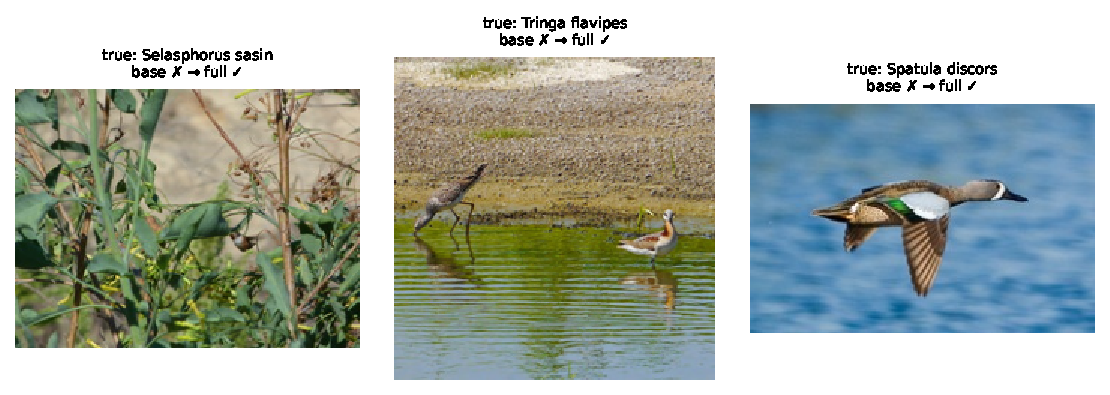
\includegraphics[width=\columnwidth]{figures/fig6_qualitative.pdf}
\caption{\textbf{Corrections.} Test samples the lower-order model gets wrong and the full model
gets right (ConFu++, seed 1): 226 net corrections.}
\label{fig:qual}
\end{figure}

\paragraph{End-to-end replication.} Jointly training encoders, fusion, and objectives (3 seeds,
identical schedule and inference capacity) shows every arm converging to \emph{text dominance}
(text drop ${+}4.9$\pp; image ${\approx}0$; audio $0$): the task loss absorbs the caption-name
leakage and the optimizer abandons the image. Accuracy is flat across arms
($71.87{\to}72.32$, ns) while de-shortcutting stays monotone
($R^2(\mathrm{text}{\to}z_{13})$: $0.81{\to}0.73{\to}0.68$). A causal control settles the
attribution: retraining all arms on name-scrubbed captions (0\% residual leakage) leaves text
dominance unchanged (drop $+5.6$\pp, acc ${\approx}72\%$) --- the dominance is intrinsic to
how informative visual descriptions are for fine-grained species ID, not to name leakage.
End-to-end, the gap manifests as \emph{modality abandonment} --- a stronger failure mode our
diagnostics expose directly.

\section{Methodology Pitfalls}\label{sec:pitfalls}
\begin{figure}[t]
\centering
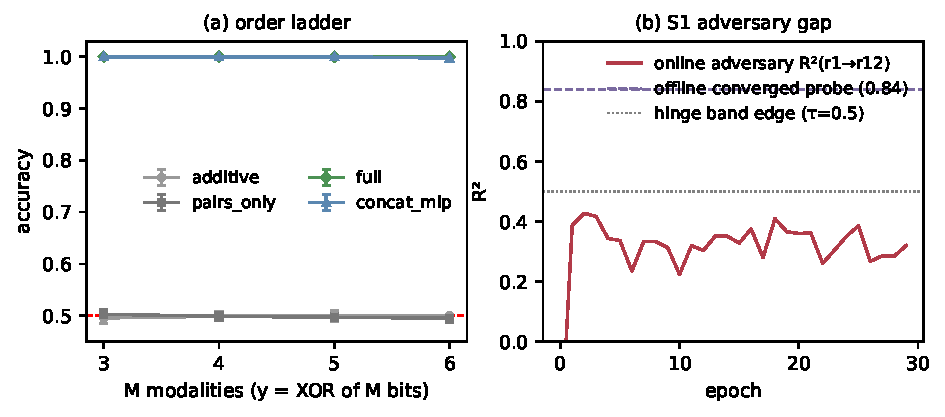
\includegraphics[width=\columnwidth]{figures/fig5_ladder_adversary_gap.pdf}
\caption{\textbf{(a)} Order ladder: order-restricted models at chance at every $M$.
\textbf{(b)} The adversary gap: the online adversary equilibrates below the hinge band while a
converged offline probe reads $R^2{=}0.84$.}
\label{fig:ladder}
\end{figure}

\textbf{Post-aggregation LayerNorm is a hidden higher-order term.} A LayerNorm applied after
summing per-modality terms divides by a cross-modal statistic: on 3-bit parity, an additive model
with a final LayerNorm reaches $0.75$ while the same model without it sits at exactly $0.50$
(all seeds, converged). Any ``low-order ablation'' ending in LayerNorm is not low-order. This
pitfall directly applies to gated-composition designs (including ours) when used as ablations.

\textbf{The adversary gap.} An online adversary updated once per batch equilibrates at
$R^2{\approx}0.3$--$0.4$ (Fig.~\ref{fig:ladder}b), below the hinge band, while a converged
offline probe still reads $0.84$. De-shortcutting claims must therefore be measured with
converged probes, not training-time meters; and residual single-modality predictability under S1
is bounded jointly by $\tau$ and this gap.

\section{Discussion}
The causal chain is complete. Where higher-order information is absent or dominated (AV-MNIST,
MOSI, UR-FUNNY), interactions shortcut; where it exists and is observable (synthetic), the
order-matched interaction extracts it completely; where it exists naturally (Bird-MML), the
original objective leaves it unused and ConFu++ recovers a significant share --- honestly, with
no fabricated dependence on the null modality, and at zero inference cost.

\textbf{Limitations.} (i) The pair-conditional gain of individual interaction terms remains
slightly negative; utility currently arrives via the jointly trained full head --- per-pair
utility objectives are the next step. (ii) Bird-MML results use a 71-species subset (upstream
release bug) and frozen features for the main matrix; the end-to-end replication is
leakage-dominated, so a de-leaked-caption retrain is the natural follow-up. (iii) All
predictability statements are operational approximations, not information-theoretic quantities.
(iv) S1's guarantee is a hinge band, not zero redundancy.

\textbf{Broader impact.} Deployed ``multimodal'' systems may silently ignore a modality
(clinical audio, accessibility channels). A dependence audit such as ours is a cheap,
transferable pre-deployment check.

\section*{Reproducibility statement}
Five seeds, paired statistics, capacity-matched probes, train-only parameter accounting, fixed
splits, git-state logging per run, and release of code, configs, the synthetic benchmark, the
diagnostic suite, and the complete experiment log (including all negative results).

{\small
\bibliographystyle{ieee_fullname}
\begin{thebibliography}{16}\itemsep1pt
\bibitem{confu} S.~Koutoupis, M.~A. Zervou, K.~Kontras, M.~De~Vos, P.~Tsakalides, and
G.~Tsagkatakis. The more, the merrier: Contrastive fusion for higher-order multimodal alignment.
\emph{CVPR}, 2026. arXiv:2511.21331.
\bibitem{clip} A.~Radford et al. Learning transferable visual models from natural language
supervision. \emph{ICML}, 2021.
\bibitem{symile} A.~Meyer et al. Symile: A total correlation objective for multimodal
contrastive learning. \emph{ICML}, 2024.
\bibitem{imagebind} R.~Girdhar et al. ImageBind: One embedding space to bind them all.
\emph{CVPR}, 2023.
\bibitem{multibench} P.~P. Liang et al. MultiBench: Multiscale benchmarks for multimodal
representation learning. \emph{NeurIPS Datasets and Benchmarks}, 2021.
\bibitem{multiviz} P.~P. Liang et al. MultiViz: An analysis benchmark for multimodal
interactions. 2022.
\bibitem{pid} P.~L. Williams and R.~D. Beer. Nonnegative decomposition of multivariate
information. 2010.
\bibitem{wang2020} W.~Wang, D.~Tran, and M.~Feiszli. What makes training multi-modal
classification networks hard? \emph{CVPR}, 2020.
\bibitem{ogm} X.~Peng et al. Balanced multimodal learning via on-the-fly gradient modulation.
\emph{CVPR}, 2022.
\bibitem{underspec} A.~D'Amour et al. Underspecification presents challenges for credibility in
modern machine learning. \emph{JMLR}, 2022.
\bibitem{dann} Y.~Ganin and V.~Lempitsky. Unsupervised domain adaptation by backpropagation.
\emph{ICML}, 2015.
\bibitem{learningnottoplearn} B.~Kim et al. Learning not to learn: Training deep neural networks
with biased data. \emph{CVPR}, 2019.
\bibitem{vicreg} A.~Bardes, J.~Ponce, and Y.~LeCun. VICReg: Variance-invariance-covariance
regularization for self-supervised learning. \emph{ICLR}, 2022.
\bibitem{lmf} Z.~Liu et al. Efficient low-rank multimodal fusion with modality-specific factors.
\emph{ACL}, 2018.
\bibitem{focal} T.-Y. Lin et al. Focal loss for dense object detection. \emph{ICCV}, 2017.
\bibitem{ast} Y.~Gong, Y.-A. Chung, and J.~Glass. AST: Audio spectrogram transformer.
\emph{Interspeech}, 2021.
\end{thebibliography}
}

\appendix
\section{Per-seed tables and failed objectives}
All five-seed runs report individual seed values in the released JSON artifacts. We additionally
document the retired objectives: P1 (conditional utility alone; improved nonlinear conditional
gain $+0.294{\pm}0.162$\pp\ on AV-MNIST without dependence) and P2 (task-aware ranking; failed
because corrupted $\approx$ positive under shortcut), and S4 (hard-fraction emphasis;
exploratory-negative, trades easy-fraction accuracy).

\section{Unit tests and protocol enforcement}
Every loss/module ships with tests for shapes, finite outputs/gradients, batch-size 1,
stop-gradient correctness (no gradient into adversaries from the generator step; none into the
interaction from the adversary step), hinge boundary behavior, and probe train/test leakage.
The statistical protocol (validation-only selection, confirmatory vs exploratory tiers, paired
tests) is enforced by the shared experiment harness.

\section{Compute}
Frozen-feature experiments: minutes per seed on one GPU. End-to-end Bird-MML arm: ${\approx}$1.5h
per seed on an RTX 5000 Ada. Synthetic suite: CPU-minutes. S1 adds 263k training-only parameters
(adversaries), zero at inference.
\end{document}
